%!TEX ROOT=sample-thesis.tex
%!TEX PROGRAM=xelatex

%%%%%%%%%%%%%%%%%%
%% Sample thesis using umsthesis.cls, August 4, 2016.
%% by Lian Tze LIM (liantze@gmail.com)
%% http://liantze.penguinattack.org/latextypesetting.html#umsthesis
%%
%% Possible options:
%% english     -- Thesis in English (default).
%% bahasam     -- Thesis in Bahasa Malaysia.
%% usesansmath -- Uses Tahoma for alphabetic math symbols too
%% microtype   -- Even nicer typographic output! Reduces chances of hyphenation
%%                but *sometimes* (though rare) may cause an endless loop as
%%                the typesetting engine tries to find an optimal line break.
%%%%%%%%%%%%%%%%%%
\documentclass[microtype]{umsthesis}
% \documentclass[microtype,bahasam]{umsthesis}

%% Theses in Bahasa Malaysia may use another style;
%% consult your faculty/school and change accordingly
\usepackage[natbibapa]{apacite}
\setcitestyle{notesep={: }}
\apptocmd{\bibfont}{\SingleSpacing}{}{}
\setlength{\bibsep}{\onelineskip}
\bibliographystyle{apacite}

%% Load any other packages you need here
\usepackage{graphicx}
%% Very useful if you're in engineering, chemistry, physics
\usepackage{siunitx}
%% Various symbols (e.g. musical notes)
\usepackage{wasysym}

%% Just for generating dummy text.
\usepackage{lipsum}

% %% Information about your thesis
\author{Lim Lian Tze}
\matric{PK00001}
\title{\LaTeX{} Thesis Template for Universiti Sabah Malaysia}
\degree{Doctor of Philosophy}
\studyfield{Computer Science}
\faculty{Faculty of Engineering}
\submissionyear{2016}
% \submissionmonth{March}
\vivadate{20 May 2016}

\begin{document}
\frontmatter

%% Generates the cover page, a blank page, and then the title page
\makecoverandtitlepage

%% Candidate's Declaration (remember to sign!)
\makedeclaration{1 Aug 2016}

%% Supervisor's Declaration (remember to sign!)
\begin{SVdeclaration}
  \member{Main Supervisor}{Name of Supervisor}
  \member{Co-Supervisor}{Name of Co-supervisor}
\end{SVdeclaration}



%% Acknowledgements in a separate file
%!TEX ROOT=sample-thesis.tex
%!TEX PROGRAM=xelatex

\begin{acknowledgement}[August 2016]
I would like to express my deepest gratitude\ldots
\end{acknowledgement}

%% English and Malay abstracts in their respective files
\inputEnAbstract{sample-abstract}
\inputMsAbstract[Nyatakan Tajuk Bahasa Malaysia]{sample-msabstract}


%% Content lists
{\clearpage\SingleSpacing
\tableofcontents\clearpage
\listoftables\clearpage
\listoffigures\clearpage
\listofphotos\clearpage
\chapter{List of Abbreviations}

{\renewcommand{\arraystretch}{2}
\begin{tabular}{@{} >{\bfseries}l l@{}}
ACM & Association of Computational Machinery\\
IR & Information Retrieval\\
NHS & National Health Service\\
WWW & World Wide Web\\
\end{tabular}
}\clearpage
\chapter{List of Symbols}

{\renewcommand{\arraystretch}{2}
\begin{tabular}{@{} >{\bfseries\boldmath }l @{\hspace{1em}--\hspace{1em}} l@{}}
$\theta$ & temperature\\
$G$ & Gravitational acceleration $= \SI{9.81}{\meter\per\second}$
\end{tabular}
}\clearpage
%!TEX ROOT=sample-thesis.tex
%!TEX PROGRAM=xelatex

\chapter{List of Musical Notations}

{\renewcommand{\arraystretch}{2}
\begin{tabular}{@{} l @{\hspace{1em}--\hspace{1em}} l@{}}
\LARGE\fullnote & semibreve\\
\LARGE\halfnote & minim\\
\LARGE\quarternote & crochet\\
\LARGE\eighthnote & quaver\\
\end{tabular}
}\clearpage
\listofappendices\clearpage
}



\mainmatter


%% Recommended to put chapters in separate files
%!TEX ROOT = sample-thesis.tex
\chapter{Introduction}

So this is the preamble at the beginning of the chapter. The purpose may be to introduce the themes of the chapter and main headings.

So this is a second paragraph.

\section{First Test and I need a really long title, please do oblige me won't you? Just a few more words and yes we're there}
\lipsum[1-2]

\begin{figure}[hbt!]\centering

\includegraphics[width=.3\textwidth]{green}
\caption[First figure]{First figure\\\source{Somewhere from the Web.}}

\bigskip

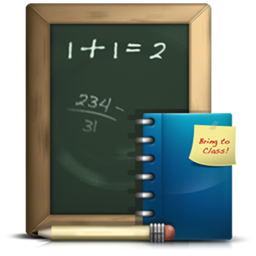
\includegraphics[width=.3\textwidth]{school}
\caption{Second figure. Now I need a long caption to test out how things look in the List of Figures. Is this long enough yet? Is it? Is it?}
\end{figure}

\lipsum[4-5]

\begin{figure}[hbt!]
\centering
%
\begin{minipage}{0.3\textwidth}
\centering

\includegraphics[width=\linewidth]{green}
\subcaption{The first subfigure}
\end{minipage}
%
\hspace{1cm}
%
\begin{minipage}{0.3\textwidth}
\centering
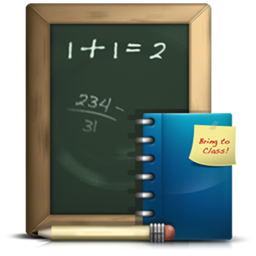
\includegraphics[width=\linewidth]{school}
\subcaption{The second subfigure}
\end{minipage}

\caption{An example with subfigures}
\end{figure}

\subsection{Second Test}
Their \cite{audibert:2004} requirements\footnote{See here, how weird, how to fill out an entire line. See here, how weird, how to fill out an entire line. See here, how weird, how to fill out an entire line. See here, how weird, how to fill out an entire line. See here, how weird, how to fill out an entire line. } are really amazing\footnote{don't you agree?} \cite[34]{budanitsky:hirst:2006}.

Looks like everyting's working. 

\begin{photo}[hbt!]
\centering
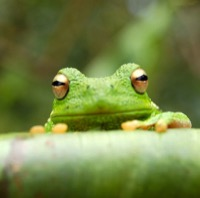
\includegraphics[width=.5\linewidth]{frog}
\caption{This is a photograph}
\end{photo}

\subsection{This is another Subsection}

Dummy text! \lipsum[1]

\section{Yeah}

And here's a long quotation, it should be an indented block and single-spaced:

\begin{quote}
\lipsum[5-6]
\end{quote}

Time for some maths, and later there's a table.

\begin{equation}
\left[M\frac{\partial }{\partial M}+\beta(g)\frac{\partial }{\partial g}+n\gamma\right] G^{(n)}(x_1,x_2,\ldots,x_n;M,g)=0
\end{equation}

\begin{table}[hbt!]
\caption{This is a table}
\centering
\begin{tabular}{ l c r }
\hline
Hey & How's it & Going?\\ \hline
Fine! & Just great. & See ya!\\
Fine! & Just great. & See ya!\\
\hline
\end{tabular}

\source{The Source.}
\end{table}

\lipsum[7]
%!TEX ROOT=sample-thesis.tex
%!TEX PROGRAM=xelatex

\chapter{Dummy Chapter with a Very Long Title to Test Spacing, So Just Bear with Me}

Hello!!

\begin{figure}[hbt!]
\centering
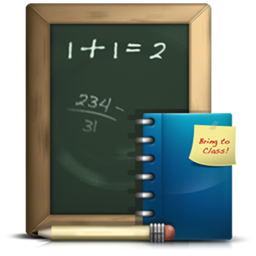
\includegraphics[width=.3\textwidth]{school}
\caption{Let's see. What have we got here?}
\end{figure}


%% Your .bib bibliography file (without .bib extension)
\bibliography{myrefs}

%% Glossary (optional)
%!TEX ROOT=sample-thesis.tex
%!TEX PROGRAM=xelatex

\chapter*{Glossary} % Chapter heading without number
\addcontentsline{toc}{chapter}{Glossary} % Add entry to ToC

{\renewcommand{\arraystretch}{2}\SingleSpacing
\begin{tabularx}{\textwidth}{@{} l @{\hspace{2em}} >{\raggedright\arraybackslash}X@{}}

dendrite & a short branched extension of a nerve cell, along which impulses received from other cells at synapses are transmitted to the cell body\\

diastole & the phase of the heartbeat when the heart muscle relaxes and allows the chambers to fill with blood.\\

\end{tabularx}
}


% %% Recommended to put appendices in separate files
\appendix
%!TEX ROOT=sample-thesis.tex
%!TEX PROGRAM=xelatex

\chapter{Manuals, Technical Specifications, Documentations, Example Scenarios}

%!TEX ROOT=sample-thesis.tex
%!TEX PROGRAM=xelatex

\chapter{Try}

\lipsum[1-2]


\end{document}